% Copyright (C) 2014-2016 by Thomas Auzinger <thomas@auzinger.name>

\documentclass[draft,final]{vutinfth} % Remove option 'final' to obtain debug information.

% Load packages to allow in- and output of non-ASCII characters.
\usepackage{lmodern}        % Use an extension of the original Computer Modern font to minimize the use of bitmapped letters.
\usepackage[T1]{fontenc}    % Determines font encoding of the output. Font packages have to be included before this line.
\usepackage[utf8]{inputenc} % Determines encoding of the input. All input files have to use UTF8 encoding.

% Extended LaTeX functionality is enables by including packages with \usepackage{...}.
\usepackage{amsmath}    % Extended typesetting of mathematical expression.
\usepackage{amssymb}    % Provides a multitude of mathematical symbols.
\usepackage{mathtools}  % Further extensions of mathematical typesetting.
\usepackage{microtype}  % Small-scale typographic enhancements.
\usepackage[inline]{enumitem} % User control over the layout of lists (itemize, enumerate, description).
\usepackage{multirow}   % Allows table elements to span several rows.
\usepackage{booktabs}   % Improves the typesettings of tables.
\usepackage{subcaption} % Allows the use of subfigures and enables their referencing.
\usepackage[ruled,linesnumbered,algochapter]{algorithm2e} % Enables the writing of pseudo code.
\usepackage[usenames,dvipsnames,table]{xcolor} % Allows the definition and use of colors. This package has to be included before tikz.
\usepackage{nag}       % Issues warnings when best practices in writing LaTeX documents are violated.
\usepackage{todonotes} % Provides tooltip-like todo notes.
\usepackage{hyperref}  % Enables cross linking in the electronic document version. This package has to be included second to last.
\usepackage[acronym,toc]{glossaries} % Enables the generation of glossaries and lists fo acronyms. This package has to be included last.

% Define convenience functions to use the author name and the thesis title in the PDF document properties.
\newcommand{\authorname}{Simon Mulser} % The author name without titles.
\newcommand{\thesistitle}{Simulation of different selfish mining strategies in Bitcoin} % The title of the thesis. The English version should be used, if it exists.

% Set PDF document properties
\hypersetup{
    pdfpagelayout   = TwoPageRight,           % How the document is shown in PDF viewers (optional).
    linkbordercolor = {Melon},                % The color of the borders of boxes around crosslinks (optional).
    pdfauthor       = {\authorname},          % The author's name in the document properties (optional).
    pdftitle        = {\thesistitle},         % The document's title in the document properties (optional).
    pdfsubject      = {Subject},              % The document's subject in the document properties (optional).
    pdfkeywords     = {a, list, of, keywords} % The document's keywords in the document properties (optional).
}

\setpnumwidth{2.5em}        % Avoid overfull hboxes in the table of contents (see memoir manual).
\setsecnumdepth{subsection} % Enumerate subsections.

\nonzeroparskip             % Create space between paragraphs (optional).
\setlength{\parindent}{0pt} % Remove paragraph identation (optional).

\makeindex      % Use an optional index.
\makeglossaries % Use an optional glossary.
%\glstocfalse   % Remove the glossaries from the table of contents.

% Set persons with 4 arguments:
%  {title before name}{name}{title after name}{gender}
%  where both titles are optional (i.e. can be given as empty brackets {}).
\setauthor{}{\authorname}{BSc}{male}
\setadvisor{}{Edgar Weippl}{Privatdoz. Mag.rer.soc.oec. Dipl.-Ing. Dr.techn.}{male}

% For bachelor and master theses:
\setfirstassistant{}{Aljosha Judmayer}{Univ.Lektor Dipl.-Ing.}{male}

% For dissertations:
\setfirstreviewer{Pretitle}{Forename Surname}{Posttitle}{male}
\setsecondreviewer{Pretitle}{Forename Surname}{Posttitle}{male}

% For dissertations at the PhD School and optionally for dissertations:
\setsecondadvisor{Pretitle}{Forename Surname}{Posttitle}{male} % Comment to remove.

% Required data.
\setaddress{Dadlergasse 18/1/7, 1150 Wien}
\setregnumber{01027478}
\setdate{13}{10}{2017} % Set date with 3 arguments: {day}{month}{year}.
\settitle{\thesistitle}{Simulation of different selfish mining strategies in Bitcoin} % Sets English and German version of the title (both can be English or German).
\setsubtitle{Simulation respecting network topology and reference implementation}{Simulation respecting network topology and reference implementation} % Sets English and German version of the subtitle (both can be English or German).

% Select the thesis type: bachelor / master / doctor / phd-school.
% Bachelor:
%\setthesis{bachelor}
%
% Master:
\setthesis{master}
\setmasterdegree{dipl.} % dipl. / rer.nat. / rer.soc.oec. / master
%
% Doctor:
%\setthesis{doctor}
%\setdoctordegree{rer.soc.oec.}% rer.nat. / techn. / rer.soc.oec.
%
% Doctor at the PhD School
%\setthesis{phd-school} % Deactivate non-English title pages (see below)

% For bachelor and master:
\setcurriculum{Software Engineering \& Internet Computing}{Software Engineering \& Internet Computing} % Sets the English and German name of the curriculum.

% For dissertations at the PhD School:
\setfirstreviewerdata{Affiliation, Country}
\setsecondreviewerdata{Affiliation, Country}


\begin{document}

\frontmatter % Switches to roman numbering.
% The structure of the thesis has to conform to
%  http://www.informatik.tuwien.ac.at/dekanat

\addtitlepage{naustrian} % German title page (not for dissertations at the PhD School).
\addtitlepage{english} % English title page.
\addstatementpage

\begin{danksagung*}
Ich möchte mich herzlichst bei meinen Eltern Theresia Jud Mulser und Josef Mulser für deren unermessliche Unterstützung während meiner gesamten Ausbildung bedanken.
Ohne ihr tiefestes Vertrauen in mich und meine Fähigkeiten hätte ich nie die Möglichkeit gehabt diesen Erfolg in meiner akademischen Karriere zu erreichen.
Weiters möchte ich mich bei meiner Freundin Julia Gatterer für den starken Rückhalt in schwierigen Phasen sowie für das Fehlerlesen dieser Arbeit bedanken.

\bigskip

Ein spezieller Dank geht auch an die Internet Privatstiftung Austria für die Förderung meiner Abschlussarbeit.
Dank dieser Förderung hatte ich die Möglichkeit mehr Zeit und Ressourcen in meine Arbeit zu investieren.
Zusätzlich konnte ich meine implementierte Simulationssoftware für allgemeinere Zwecke erweitern und als alleinstehendes Framework für weitere Entwicklung und Forschung zur Verfügung stellen.

Abschließend möchte ich mich bei Privatdoz. Mag.rer.soc.oec. Dipl.-Ing. Dr.techn. Edgar Weippl und Univ.Lektor Dipl.-Ing. Aljosha Judmayer für die Möglichkeit zum Verfassen dieser Diplomarbeit sowie für das konstruktive Feedback und die aufmerksame Betreuung bedanken.

\end{danksagung*}

\begin{acknowledgements*}
First, I would like to sincerely thank my parents Theresia Jud Mulser and Josef Mulser for their ongoing support throughout my whole education. Without their endless trust in and my abilities, I would have never had the opportunity to reach this point in my academical career. Furthermore, I thank my girlfriend Julia Gatterer for her tireless motivation during critical phases and for the review of the present work.

Special thanks go to Internet Foundation Austria for granting me a scholarship for this thesis. With the scholarship, I had the possibility to invest more time and resources in the thesis. Additionally, I could adopt the implemented software for a more general purpose and provide it as a stand-alone framework to foster more investigation and development in the research area.

Finally, I would like to thank Privatdoz. Mag.rer.soc.oec. Dipl.-Ing. Dr.techn. Edgar Weippl and Univ.Lektor Dipl.-Ing. Aljosha Judmayer for the possibility of conducting this master thesis and their supervision during the creation of the thesis.

\end{acknowledgements*}

\begin{kurzfassung}
Die Cryptocurrency Bitcoin wurde im Jahre 2008 mit dem Erstellen des ersten Blocks, dem Genesis Block, gestartet.
Seitdem hat sich die Rechenleistung des Netzwerkes, welches die Blockchain der digitalen Währung absichert, erheblich vervielfacht.
Heutzutage erweitern um die zwanzig professionelle Miner laufend die Blockchain, indem sie immer auf den jeweils neuesten, ihnen bekannten Block aufbauen.
Die Miner belohnen sich dabei selbst, da sie mit jedem erstellten Block für sich neue Bitcoins schürfen.
Im Jahre 2014 zeigte Eyal und Gün Sirer erstmals dass es neben diesem gewünschtem, ehrlichen Verhalten abweichende Miningmethoden gibt, welche den relativen Ertrag eines Miners gegenüber seiner Kontrahenten erhöht.\\
Dieser sogenannte Selfish-Mining-Angriff und all seine	 Modifikationen werden in der vorliegenden Diplomarbeit untersucht und mit bisherigen Forschungsresultaten verglichen.
Im Gegensatz zu den bisherigen Forschungsarbeiten wird dafür eine neuartige, deterministische Simulationsmethode verwendet, welche das zugrunde liegende Peer-to-Peer-Netzwerk und alle Eigenschaften des Bitcoin-Protokolls akkurater abbildet.
Dies wird ermöglicht, indem das gesamte Netzwerk mittels der Software \textit{Docker} virtualisiert wird.
Dadurch wird der Netzwerklayer des Systems und dessen Latenz auf natürliche Art und Weise nachgebildet.
Weiteres kann das Bitcoin-Protokoll realitätsnah simuliert werden, da die Referenzimplementierung direkt in den Nodes des Netzwerkes ausgeführt wird.\\
%Neben der Berücksichtigung aller Details des Protokolls erspart man sich dabei zusätzlich eine fehleranfällige und zeitaufwendige Adaptierung oder Neuimplementierung des Protokolls.\\
Die Resultate der Simulationen zeigen die jeweils effizienteste Selfish-Mining-Strategie für eine bestimme Rechenleistung des Angreifers und untermauern den momentanen Forschungsstand sowie die Relevanz des Selfish-Mining-Angriffs.
Weiters wurde durch die implementierte Simulationsmethode ein neues Simulationsframework entwickelt, welches das Erforschen verschiedenster Angriffsvektoren und Testen von Verbesserungen unterschiedlicher Blockchain-Protokolle erleichtert.

\bigskip
\noindent \textbf{Schlagwörter}\\
Selfish-Mining, Selfish-Mining-Angriff, Bitcoin, Blockchain, Simulation, Simulationsmethode, Simulationsframework, Netzwerklatenz, Referenzimplementierung, Docker

\end{kurzfassung}

\begin{abstract}
The Cryptocurrency Bitcoin was started in 2008 with the creation of the first block, the Genesis Block. 
Since then, the computing power of the network, which secures the blockchain of the digital currency, has multiplied considerably.
Today, around twenty professional mining pools share over $ 95\% $ of the hash rate, and are constantly extending the blockchain, always building on the latest block known to them.
The miners are incentivised to do so, as they create with each
found block new Bitcoins for themselves.\\
In 2014, Eyal and Gün Sirer showed for the first time that apart from this desired, honest behaviour, there are deviating mining methods that increase the relative gain of a miner compared to the rest of the network.
This so-called selfish mining attack and all its modifications are examined in this thesis in a defined scenario with twenty miners and are compared with previous research results.
In contrast to previous investigations, a novel, deterministic simulation framework based on \textit{Docker} was developed for this purpose.
This simulation framework makes it possible to naturally include the network latency and to directly reuse the reference implementation of Bitcoin.
The latter has the advantage that no time-consuming and error-prone adaptation or abstraction of the reference implementation is necessary and all properties of the implemented Bitcoin protocol are automatically included in the simulation.
To simulate the various selfish mining strategies, additionally, a proxy was implemented that eclipsed a node in the network and misuses the node to perform the various selfish mining attacks.\\
The simulations of the various selfish mining strategies show that a dishonest miner can increase its relative gain over the rest of the network, thus reinforcing the current state of research and the relevance of the selfish mining attack.
In accordance with previous results, the most efficient selfish mining strategies under the simulation scenario with twenty miners, selfish mining and equal-fork-stubbornness were identified.

\bigskip
\noindent \textbf{Keywords}\\
selfish mining, selfish mining attack, Bitcoin, blockchain, simulation, simulation framework, network latency, reference implementation, Docker

\end{abstract}

% Select the language of the thesis, e.g., english or naustrian.
\selectlanguage{english}

% Add a table of contents (toc).
\tableofcontents % Starred version, i.e., \tableofcontents*, removes the self-entry.

% Switch to arabic numbering and start the enumeration of chapters in the table of content.
\mainmatter

\chapter{Introduction}
The cryptocurrency Bitcoin started back in the year 2008 with the release of the Bitcoin white paper \cite{nakamoto2008bitcoin}.
As of today, the cryptocurrency has reached a market capitalization of over 20 billion dollars \cite{marketcap2017}.
Internally the Bitcoin cryptocurrency records all transactions in a public ledger called \emph{blockchain}.
The blockchain is basically an immutable linked list of blocks where a block contains multiple transactions of the cryptocurrency.
In Bitcoin, each block needs to contain a so-called proof of work (PoW) which is the solution to a costly and time-consuming cryptographic puzzle.
Miners connected in a peer-to-peer network compete with their computation power to find solutions to the puzzle and hence to find the next block for the blockchain.
Finding a block allows the miners to add a transaction to the block which gives them certain amount of bitcoins.
Additionally, the grouping of the transactions in blocks creates a total order and hence makes it possible to prevent double-spending.
After a block is found by a miner, all other miners should adopt to this new tip of the chain and try to find a new block on top.
This mining process is considered as incentive compatible as long as no single miner has more than 50\% of the total computation power.

\cite{eyal2014majority} showed that also miners under 50\% have an incentive to not follow the protocol as described depending on their connectivity and share of computation power in the peer-to-peer network.
By conducting a so-called selfish mining strategy a miner can obtain relatively more revenue than its actual proportion of computational power in the network.
In general, the miner simply does not share found blocks with the others and secretly mines on its own chain.
If its chain is longer then the public chain, it is able to overwrite all blocks found by the honest miners.
If the two chains have the same length the private miner also publishes its block and causes a block race.
Now the network is split into two parts where one part is mining on the public tip and the other part is mining on the now public-private tip.
In general, the selfish miner achieves that the other miners are wasting their computational power on blocks which will not end up in the longest chain and thus is able to increase its relative share of mining rewards.

\todo[inline]{explained relative gain/total gain}

Even though the selfish miner can increase is relative gain in respect to the other miners, its total gain is lower than it would behave honest.
This is possible because the execution of the selfish mining algorithm by the selfish miner decreases the amount of blocks which end up in the longest chain.
During the selfish mining more blocks by both, the selfish miner and the honest network, are not included in the longest chain, so-called stale blocks.
Hence, less mining rewards are distributed between the nodes in the network which also affects the miner conducting selfish mining.
The fact that less mining rewards are distributed prevails the relative gain obtained by selfish miner and therefore the selfish miner earns less than it would earn behaving honestly \cite{nayak2016stubborn, sapirshtein2016optimal}.
Since there end up less blocks in the longest chain the Bitcoin protocol would simplify the cryptographic puzzle during the next difficulty adjustment.
From then on more blocks are found and it is likely that the selfish miner would also increase its total gain.
The scenario where the difficulty is adjusted was not yet investigated by researchers and is also not a focus of this thesis.

Despite the normal selfish mining further research \cite{nayak2016stubborn,sapirshtein2016optimal, gervais2015tampering, gervais2016security, bahack2013theoretical} showed different modifications of the algorithm which perform slightly better under certain circumstances.
These modifications include for example the idea that the selfish miner does not adopt immediately to new blocks but trails behind the public chain and tries to catch up with its secretly mined, private chain.
Furthermore, the selfish mining attack can be combined with different other attacks such as double spending increasing the gain of the misbehaving miner \cite{gervais2016security, sapirshtein2016optimal, nayak2016stubborn, gervais2015tampering}.

To prove the existence and attributes of selfish mining different approaches were applied.
The researchers used simple probabilistic arguments \cite{eyal2014majority, bahack2013theoretical}, numeric simulation of paths with state machines \cite{gervais2015tampering, nayak2016stubborn}, advanced Markov Decision Processes (MDP) \cite{sapirshtein2016optimal, gervais2016security} or gave results of closed-source simulations \cite{eyal2014majority, sapirshtein2016optimal}.
Unfortunately, we cannot discuss the closed source simulations in detail.
All other above-mentioned methodologies have the following drawbacks:
\begin{itemize}
\item Abstraction of the Bitcoin reference implementation which runs inside a node of the peer-to-peer network.
Since there is no official specification of the Bitcoin protocol it is hard to capture all details.
Furthermore, it is hard to keep the simulation framework up-to-date because of the ongoing development of the protocol.
\item Abstraction of the whole network layer of the peer-to-peer network.
The available simulations abstract the network topology by either defining a single connectivity parameter \cite{eyal2014majority, bahack2013theoretical, nayak2016stubborn, sapirshtein2016optimal, gervais2015tampering} or by using the stale block rate as input for the MDP \cite{gervais2016security}.
Hence the highly abstract the presence of network delays and natural forks of the chain.
\end{itemize}

\todo[inline]{first usage of "stale block rate", but with a reference. detailed explanation of relative gain later in the thesis}

In this thesis, we propose a new simulation approach which tackles this two drawbacks and hence captures more accurately the details of the Bitcoin reference implementation and the whole network layer while allowing for a high degree of determinism.
The introduced simulation approach is then used to examine the following selfish mining strategies:

\begin{itemize}
\item selfish mining \cite{eyal2014majority}
\item lead stubborn mining \cite{nayak2016stubborn}
\item trail stubborn mining \cite{nayak2016stubborn}
\item equal-fork stubborn mining \cite{nayak2016stubborn}
\end{itemize}

These strategies are executed by a selfish mining node in a defined, realistic simulation scenario with a certain amount of participating nodes.
To gain a holistic insight different distributions of computation power between the nodes are used.

The result of the executed simulations shows which strategy is the best strategy for a certain distribution of mining power between the selfish miner and the honest network.
Furthermore, the relative and total gain of the selfish miner in the different simulation scenarios is observed. The outcome of the thesis is further analysed by answering the following two research questions:

\begin{itemize}
	\item \textbf{RQ1:} Do the simulations of selfish mining with the proposed software solutions show an increase of the total and relative gain for the selfish miner compared to the normal, honest mining behaviour?

	\item \textbf{RQ2:} How does the obtained results of the simulation match the outcome of previous research in the area of selfish mining?
\end{itemize}


An additional outcome of the thesis is a general simulation framework.
The framework allows an accurate and deterministic simulation of the blockchain by using directly the reference implementation and a realistic network topology.
Hence, the simulation framework could not only be used to simulate selfish mining attacks but could for example be used to simulate other attacks or new protocol versions of Bitcoin. 
Since many other cryptocurrencies are derived from Bitcoin, they simulation framework could also be utilized to simulate their behaviour and properties.

\section{Structure of this thesis}

\todo[inline]{reorder to reflect ToC and added paragraph for evaluation of the framework}

First, a simulation framework is implemented.
To be able to control when a certain node finds a block, all Bitcoin nodes are executed in \textit{regtest} mode.
In this test mode, the real PoW-algorithm is disabled and every node accepts a command which lets the node create immediately a new block.
With this functionality, it is possible to define a block discovery series which basically reflects the computation power of each node.
The more blocks are found by a node the more simulated computation power the node has.
Additionally to the block generation, the simulation framework also controls the network topology and hence the connectivity of each node.
For the simulation run, it is important that the connectivity of the nodes stays the same to make the results better comparable.
This is achieved by setting the connections from the nodes by the simulation framework itself which is in contrast to the normal behaviour.
Normally Bitcoin nodes share their connections with other nodes over the Bitcoin protocol and try to improve the connectivity over time.

Subsequently, the determinism of the simulation framework is evaluated.
Therefore a deterministic behaviour and a realistic reference scenario reflecting the Bitcoin network is defined.
The results of executing the scenario with the framework show then that the framework behaves deterministically as defined. 

In the next step, the different strategies selfish, lead stubborn, trail stubborn and equal-fork stubborn mining from \cite{nayak2016stubborn} and \cite{eyal2014majority} are implemented.
This is achieved by implementing a proxy which eclipses a normal Bitcoin client from the other nodes in the network.
Now, if a block is found the proxy decides, depending on its selfish mining strategy, if a block should be transmitted from the eclipsed node to the rest of the network or vice versa.
The proxy design pattern makes it possible to implement the selfish mining strategies without altering the reference implementation of Bitcoin and is therefore preferred over an implementation directly in the Bitcoin client.

Lastly, the simulation framework and the selfish proxy is used to simulate the various selfish mining strategies.
Therefore the reference scenario defined for evaluating the framework is combined with different distributions of computation power between the selfish miner and the honest network.
The results of this simulations are then analysed and compared with previous research in this area.


\chapter{Problem}
The cryptocurrency Bitcoin started back in the year 2008 with the release of the Bitcoin white paper \cite{nakamoto2008bitcoin}.
As of today, the cryptocurrency has reached a market capitalization of over 20 billion dollars \cite{marketcap2017}.
Internally the Bitcoin cryptocurrency records all transactions in a public ledger called \emph{blockchain}.
The blockchain is basically an immutable linked list of blocks where a block contains multiple transactions of the cryptocurrency.
In Bitcoin, each block needs to contain a so-called proof of work (PoW) which is the solution to a costly and time-consuming cryptographic puzzle.
Miners connected in a peer-to-peer network compete with their computation power to find solutions to the puzzle and hence to find the next block for the blockchain.
Finding a block allows the miners to add a transaction to the block and gives them right to newly create a certain amount of bitcoins.
Additionally, the grouping of the transactions in blocks creates a total order and hence makes it possible to prevent double-spending.
After a block is found by a miner, all other miners should adopt to this new tip of the chain and try to find a new block on top.
This mining process is considered as incentive compatible as long as no single miner has more than 50\% of the total computation power.

\cite{eyal2014majority} showed that also miners under 50\% have an incentive to not follow the protocol as described depending on their connectivity and share of computation power in the peer-to-peer network.
By implementing a so-called selfish mining strategy a miner can obtain relatively more revenue than his actual proportion of computational power in the network.
In general, the miner simply does not share found blocks with the others and secretly mines on his own chain.
If his chain is longer then the public chain, he is able to overwrite all blocks found by the honest miners.
If the two chains have the same length the private miner also publishes his block and causes a block race.
Now the network is split into two parts where one part is mining on the public tip and the other part is mining on the now public-private tip.
In general, the selfish miner achieves that the other miners are wasting their computational power on blocks which will not end up in the longest chain.

Further research \cite{nayak2016stubborn,sapirshtein2016optimal, gervais2015tampering, gervais2016security, bahack2013theoretical} explored different modifications of the original selfish mining algorithm by \cite{eyal2014majority} and found slightly modifications of the algorithm which perform better under certain circumstances.
For example, it could make sense for the selfish miner to even trail behind the public chain.

To prove the existence and attributes of selfish mining different approaches were applied.
The researchers used simple probabilistic arguments \cite{eyal2014majority, bahack2013theoretical}, numeric simulation of paths with state machines \cite{gervais2015tampering, nayak2016stubborn}, advanced Markov Decision Processes (MDP) \cite{sapirshtein2016optimal, gervais2016security} or gave results of closed-source simulations \cite{eyal2014majority, sapirshtein2016optimal}.
Unfortunately, we cannot discuss the closed source simulations in detail.
All other above-mentioned methodologies have the following drawbacks:
\begin{itemize}
\item Abstraction of the Bitcoin source code which normally runs on a single node.
Since there is no official specification of the Bitcoin protocol it is hard to capture all details.
Furthermore, it is hard to keep the simulation software up-to-date because of the ongoing development of the protocol.
\item Abstraction of the whole network layer of the peer-to-peer network.
The available simulations abstract the network topology by either defining a single connectivity parameter \cite{eyal2014majority, bahack2013theoretical, nayak2016stubborn, sapirshtein2016optimal, gervais2015tampering} or by using the block stale rate as input for the MDP \cite{gervais2016security}.
Hence the highly abstract the presence of network delays and natural forks of the chain.
\end{itemize}

In this thesis, we propose a new simulation approach to more accurately capture the details of the Blockchain protocol under simulation, while allowing for a high degree of determinism.
With our simulation, it would be possible to model the selfish mining attack with different network topologies and to use the Bitcoin source code directly in the simulation.

\chapter{Expected results}
The expected outcome of this thesis is a more accurate simulation of different selfish mining strategies and therefore a better understanding of the potential real world implications of such attacks.
The selfish mining strategies used in the thesis include:
\begin{itemize}
\item selfish mining \cite{eyal2014majority}
\item lead stubborn mining \cite{nayak2016stubborn}
\item trail stubborn mining \cite{nayak2016stubborn}
\item equal-fork stubborn mining \cite{nayak2016stubborn}
\end{itemize}

For the simulation, these strategies are combined with different distributions of computation power in the underlying peer-to-peer network.
The result of the simulations should show which strategy is the best strategy for a certain distribution of mining power and if the selfish mining increases the relative gain of the selfish miner compared to the normal, honest mining.
The simulation results should emphasise the recent work in the area of selfish mining and show that the current implementation of Bitcoin protocol is vulnerable against different selfish mining strategies.

The desired outcome of the thesis is supported with the following two research questions:

\begin{itemize}
	\item \textbf{RQ1:} Do the simulations of selfish mining with the proposed software solutions show an increase of the relative gain for the selfish miner compared to the normal, honest mining behaviour?

	\item \textbf{RQ2:} How does the obtained results of the simulation match the outcome of previous research in the area of selfish mining?
\end{itemize}


An additional outcome of the thesis is the simulation software.
The software should allow an accurate and deterministic simulation of the blockchain by using directly the reference implementation and a realistic network topology.
Hence, the simulation software could not only be used to simulate selfish mining attacks but could for example also be used to simulate other attacks or new protocol versions of Bitcoin. 
Since many other cryptocurrencies are derived from Bitcoin, they simulation software could be used also to simulate their behaviour and properties.


\chapter{Methodology and Approach}
First, the different strategies selfish, lead stubborn, trail stubborn and equal-fork stubborn mining from \cite{nayak2016stubborn} and \cite{eyal2014majority} need to be implemented.
This is achieved by implementing a proxy which eclipses a normal Bitcoin client from the other nodes in the network.
Now, if a block is found the proxy decides, depending on his selfish mining strategy, if a block should be transmitted from the eclipsed node to the rest of the network or vice versa.
The proxy design pattern makes it possible to implement the selfish mining strategies without altering the reference implementation of Bitcoin and is therefore preferred over an implementation directly in the Bitcoin client.

In the next step, a simulation program is implemented.
To be able to control when a certain node finds a block, all Bitcoin nodes should be executed in \textit{regtest} mode.
In this test mode, the real PoW-algorithm is disabled and every node accepts a command which lets the node create immediately a new block.
With this functionality, it is possible to define a block discovery series which basically reflects the computation power of each node.
The more blocks are found by a node the more simulated computation power the node has.
Additionally to the block generation, the simulation program should also control the network topology and hence the connectivity of each node.
For the simulation run, it is important that the connectivity of the nodes stays the same to make the results better comparable.
This should be achieved by setting the connections from the nodes by the simulation program itself which is in contrast to normal behaviour.
Normally Bitcoin nodes share their connections with other nodes over the Bitcoin protocol and try to improve the connectivity over time.

After the implementation of the selfish mining strategies and the simulation program, the mining strategies are simulated.
Different network topologies and distributions of computation power are used to compare the relative gain of the selfish mining strategies over the normal, honest mining.


\chapter{State-of-the-art}
Already in the year 2010, the user \textit{ByteCoin} described the idea of selfish mining in the Bitcoin forum \textit{bitcointalk} \cite{ByteCoin2010}.
He provided simulation results of the attack which at that time was called \textit{mining cartel attack}.
Nevertheless, the discussions in the thread never caught fire and no further investigations or countermeasures were taken by the community \cite{BitcoinTalk2010, bahack2013theoretical}.

Later in 2014 \cite{eyal2014majority} released the paper \textit{"Majority is not enough: Bitcoin mining is vulnerable."} and coined the term selfish mining.
The paper gives a formal description of selfish mining and proves how a miner can earn more than his fair share by conducting the attack.
Figure \ref{fig:selfish_mining} shows the attack as a state machine where $\alpha$ denotes the mining power share of the selfish miner.
The labels of the states are representing the lead of the selfish miner over the public chain.
Whenever the public network finds a block and the selfish miner publishes a competing block of the same height a block race occurs denoted with the state \textit{0'}.
In the case of such a block race, the variable $\gamma$ expresses the probability of the selfish miner to win the block race.
Hence $\gamma$ part of the miners are mining on the public-private block and respectively $(1 - \gamma)$ are mining on the public block.
The labels on the transitions are representing the transition probabilities between the states.
The profitability of the simple strategy of \cite{eyal2014majority} was proven by using probability calculations based on the state machine of figure \ref{fig:selfish_mining}.
Furthermore, results of an undisclosed Bitcoin protocol simulator were given.
In the simulation, 1000 miners with the same mining power were simulated and a fraction of these miners formed a pool which applied the selfish mining algorithm.
In the case of a block race they artificially split the network where one part is mining on the public block and one part is mining on the block of the selfish pool.

\begin{figure}[t]
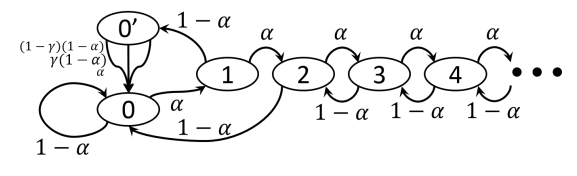
\includegraphics[width=8cm]{selfish_mining}
\centering
\caption{Selfish mining state machine with transition probabilities \cite{eyal2014majority}}
\label{fig:selfish_mining}
\end{figure}

Further research showed that more generalised selfish mining strategies lead to even more relative gain for the selfish miner \cite{nayak2016stubborn,sapirshtein2016optimal, gervais2015tampering, gervais2016security, bahack2013theoretical}.
\aju{Describe the \emph{relative gain} aspect here in one parapgraph before it is used in the above sentence. Maybe therefore first describe the term \emph{stale block rate}. Maybe start like that: One important metric in context of PoW Blockchains is the stale block rate. It ... }
The authors of \cite{nayak2016stubborn} provided a comprehensive description of the strategy space and also coined different names for the selfish mining variations:
\aju{Its better style to start a sentence with a word and not directly with a reference.}

\begin{itemize}
	\item \textbf{Lead stubborn}: 
	This mining strategy compromises the idea to cause as many block races as possible and to never overwrite the public chain with a longer chain.
	This strategy continuously tries to split the network to mine on different blocks and is therefore especially promising when the probability to win the block race is very high.
	\item \textbf{Equal-fork stubborn}: 
	The mining strategy equal-fork stubborn changes the selfish mining strategy just by one transition.
	In case the selfish miner finds a block during a block race, it does not publish his block to win the race but it also keeps this block undisclosed to secretly mine on this new tip of the chain.
\item \textbf{Trail stubborn}: 
The mining strategies based on trail stubbornness are reflecting the idea to even trail behind the public chain and to eventually catch up.
	Trail stubbornness is defined with an integer denoting how many blocks the strategy should allow the selfish miner to trail back.
\end{itemize}

The strategy space for a selfish miner is practically endless and combinations of the aforementioned strategies are possible and are leading to even more relative gain compared to honest miners \cite{nayak2016stubborn,sapirshtein2016optimal, gervais2015tampering, gervais2016security, bahack2013theoretical}.

\todo[inline]{extend to explain stale block rate}

To find the best strategy for a given mining power share $\alpha$ and connectivity $\gamma$ researchers used different methodologies.
\cite{eyal2014majority, sapirshtein2016optimal} used closed-source simulations which we cannot discuss here.
Other researchers used numeric simulations of paths in the state machine to find optimal selfish mining strategies \cite{gervais2015tampering, nayak2016stubborn}.
Lastly, \cite{sapirshtein2016optimal, gervais2016security} used MDPs based on a state machine to find strategies with the most relative gain.
The basic structure of the used state machines is for all publications the same, despite the MDP introduced by \cite{gervais2016security}.
They additionally they used in their MDP the so-called stale block rate which denotes the ratio between blocks from the consensus chain and stale blocks.
This metric accounts for the most important parameters of a blockchain protocol such as block sizes, block intervals, network delays, information propagation mechanisms and network configuration and can be seen as a general security parameter of a blockchain protocol.
The higher the stale block rate, the less secure the blockchain protocol \cite{gervais2016security}.

Besides using variations of the selfish mining strategies, the attack can also be combined with other attacks to achieve better results \cite{gervais2016security, sapirshtein2016optimal, nayak2016stubborn, gervais2015tampering}.
If the eclipse attack is used in combination with selfish mining the victim contributes its mining power to the private chain and hence, strengthens the position of the selfish miner \cite{nayak2016stubborn, gervais2016security}.
\cite{nayak2016stubborn} additionally shows that the eclipsed victim under certain circumstances can benefit from the attack and therefore has no incentive to stop the attack.
Another attack which can be used in combination with selfish mining is double-spending \cite{sapirshtein2016optimal, gervais2016security}.
Every time the selfish miner starts his selfish mining attack it can publish a transaction and include a conflicting transaction in his first secret block.
During the execution of the selfish mining attack, the payment receiver may accept the payment depending on his block confirmation time.
Now in the case of a successful selfish mining attempt, the adversary can overwrite the public chain, which additionally results in a successful double spending.
The operational costs of unsuccessful double-spending can be seen as low because the adversary still would get goods or a service in exchange for the transaction \cite{sapirshtein2016optimal, gervais2016security}.

Last but not least also the prevention of selfish mining is part of the current work in selfish mining research \cite{eyal2014majority, billah2015one, solat2016zeroblock, zhang2017publish}.
A backwards-compatible patch to mitigate selfish mining is uniform tie-breaking \cite{eyal2014majority}.
This means whenever a node receives two blocks of the same height it randomly select one of the blocks to mine on.
\cite{eyal2014majority} showed that this would raise the profit threshold to 25\% of the computational power and hence mitigating selfish mining.
The drawback of this proposed change is that it would increase the connectivity of badly connected attackers to almost 50\% with no actual effort for them.
Ethereum, the currently second largest cryptocurrency by market capitalization \cite{marketcap2017}, has implemented uniform tie-breaking as a countermeasure against selfish mining \cite{gervais2016security, unifromtiebreakingethereum}.
Another countermeasure foresees unforgeable timestamps to secure Bitcoin against selfish mining \cite{billah2015one}.
This countermeasure would make all pre-mined blocks of the selfish miner invalid after a certain amount of time.
The implementation of this patch would require random beacons and hence introduce complexity and a new attack vector \cite{billah2015one}.
\cite{zhang2017publish} proposes backwards-compatible countermeasure by neglecting blocks that are not published in time and allows incorporation of competing blocks in the chain similar to Ethereum's uncle blocks \cite{wood2014ethereum}.
This enables a new fork-resolving policy where a block always contributes to neither or both branches of the fork \cite{zhang2017publish}.
All of this mentioned countermeasures are not planned to be implemented or implemented in Bitcoin \cite{bitcoin, bitcoinbip}.
The countermeasures against selfish mining are forming an interesting research field but are not in the focus of this thesis.
Nevertheless, all of them would profit from an evaluation method introduced in the next chapter.


\chapter{Relation to curriculum}
Bitcoin and cryptocurrency technologies in general are a relatively new topic.
Hence there are no concrete subjects or modules teaching this technology in the current curriculum.
But under the hood Bitcoin technically is just a composition of different technologies which can be related to modules of the curriculum.
First of all, Bitcoin is a software acting as a distributed system and can, therefore, be linked to the modules \textit{Software Engineering} and \textit{Distributed Systems}.
Furthermore, Bitcoin uses cryptography to secure the system, which can be linked to the module \textit{Advanced Security}.
Hash functions are the main component of the PoW-algorithm in the mining process which helps to prevent double spending.
Furthermore, digital signatures based on cryptography are used to secure the bitcoins held by the different users of the system.

In the thesis, the implementation of a proxy enabling selfish mining strategies and a simulation program are carried out.
Since both of them are an implementation effort they can be directly linked to the module \textit{Software Engineering}.
Furthermore, both software programs are related to the module \textit{Distributed Systems}.
The proxy needs to be suited between multiple nodes in a Bitcoin network which is a distributed system and the simulation program needs to start-up, manage and tear-down exactly this distributed system.


\chapter{Architecture selfish proxy}
what are we doing now?
 - describing proxy \todo{okay to write what I am doing now?}
 - central point which implements selfish mining
 - relays and withholds blocks
 - not relaying tx

why we used a proxy?
 - fast implementation
 - no need to touch reference implementation

disadvanteges
 - extra hop
 - not a real proxy
   - need to keep track of chain
   - bitcoin protocol not easy

create a component diagram
 - network
 - chain
 - strategy
create a picture showing how blocks are relayed in bitcoin
\todo{any software recommendation for charts/diagrams}
 
\section{Communication}
 - how did we implement it?
   - based on pycoin of decker and python-bitcoinlib of todd
   - using gevent and hence co-routines to handle request
   - listening for incoming connections
   - private ip recognized because of unique ip
 - block relay
   - how does block relay work
   - compact blocks
   - how did we implement it
     - no compact blocks
     - assuming all blocks are valid
     - when we have the whole block pass it to chain

\section{Chain}
 - how did we implement it?
   - data structure
   - private/public highest tip
   - transfer\_allowed
   - block arrives, try to insert in chain. yes or orphaned. if yes check if orphaned can be added.
   - check if fork changed? pass it to strategy

\section{Strategy}
 - receives height of private and public
 - searches action to execute
   - 4 different types of actions (wait, adopt, match, implement)
 - executes by sending inv's
 - which strategies did we implement?
 - \todo{how works each strategy? describe it here or in section simulation and reference to the section.}
 - how did we implement it?
   - search for an action
   - if-else control structure
   - many unit tests
   


\chapter{Architecture simulation software}
what are we doing now?
 - describing the simulation software
 - simulation software exposes six commands
   - nodes
   - network
   - connectivity
   - ticks
   - simulate
   - run
   - multi-run

\section{Configuration files}

nodes
 - let you create groups of node with the same configuration
 - group has type, amount, share, latency, docker image
 - groups are persisted in a csv
 
network
 - let you create a network configuration
 - takes nodes.csv and connects them based on defined connectivity
 - network configuration is persisted in a csv

ticks
 - let you create a certain amount of ticks
 - a tick contains block events
 - using a exponential distribution and depending on the computational share it is determined when a node finds a block
 - ticks are persisted in a csv

component diagram of simulation software
 - simulationfiles
 - run, multi-run
 -  prepare
 - execution
 - post processing
 
 flow chart of run command

\section{Simulation}

 - executed eg. with simulate cmd
 - in the simulation docker is used
 - each simulation has three todo{phases/steps (which word should we use?)}
 - takes configuration files as input 

\subsection{Preparation}
 - nodes are created and connected
 - create RPC-connection
 - wait until ready
\subsection{Execution}
 - execute ticks from ticks.csv line by line
 - tick duration defined
 - execute all events in tick sequentially
 - afterwards sleep until tick is over, then start over again
 - during execution CPU \& RAM usage is collected
\subsection{Post processing}
 - get chaintips of all nodes
 - calculate consensus chain
   - start at first block height
   - request from all nodes blocks
   - if every node has a block and all blocks are the same, add block to consensus chain and heigt++
   - otherwise stop
 - stop nodes
 - process log file of every node and log file of simulation software
 - parse log events:
   - BlockCreateEvent
   - BlockStatsEvent
   - UpdateTipEvent
   - PeerLogicValidationEvent
   - TxEvent
   - TickEvent
   - BlockReceivedEvent
   - BlockReconstructEvent
   - TxReceivedEvent
   - BlockExceptionEvent
   - TxExceptionEvent
   - RPCExceptionEvent
 - pre-processing csv
   - need to have one report.rmd for run and multi-runs
   - remove skip-ticks
   - files are not sorted because of multi-processed parsing; sort by timestamp 
 - report creation
   - with Rmarkdown, R ...
   - calculate propagation time of blocks
   - calculate stale blocks
   - create useful stats about CPU \& RAM usage, duration, blocks, propagation, exceptions...
   
\subsection{Multi-runs}
 - runs a simulation multiple times with the same arguments
 - merges csv of all runs by type
 - create a report showing all results of all runs

\chapter{Near determinism of simulations}
\todo{how should we do that?}
 - we can execute simulation multiple times (100 times would last ~week)
 - then we can look at the stale block rate
 - check which distribution is appropriate
 - and then we will see :D
 https://www.researchgate.net/post/What_do_you_consider_a_good_standard_deviation
 https://stats.stackexchange.com/questions/132652/how-to-determine-which-distribution-fits-my-data-best
 http://blog.minitab.com/blog/adventures-in-statistics-2/how-to-identify-the-distribution-of-your-data-using-minitab

\chapter{Simulation of selfish mining strategies}
With the introduced software solutions, the simulation software and the selfish proxy, it is now possible to analyse selfish mining and its impact on the relative gain of the selfish miner.
For the simulation, the scenario described in chapter 45 is adapted.
One of the twenty nodes is eclipsed with the selfish proxy forming a selfish miner.
To obtain a comprehensive overview of the impact of selfish mining the selfish miners conducts various combinations of selfish mining strategies.
Additionally, different distributions of the computation power between the nodes and the selfish miner are applied.

\section{Selfish mining scenarios}

As strategies, the standard selfish mining strategy and the three modifications lead stubborn, equal-fork stubborn and trail stubborn mining are put into action.
The used trail-stubborn strategy is parametrised with 1 meaning that the selfish miner will at the maximum trail one block behind the public chain.
Hence, the at least trail stubborn strategy is executed in the different scenarios.
Since the modifications of the selfish mining strategies can be combined a total of eight different selfish mining strategies are executed during the simulation.

For the distribution of computation power, five different settings are used where the selfish miner receives either 15\%, 22.5\%, 30\%, 37.5\% or 45\% of the computation power.
The rest of the computation power in each scenario is distributed equally over all remaining, honest nodes.
The five used shares are each 7.5\% apart covering sensitive shares of the computation share.
All possible scenarios where the selfish miner would receive more than 50\% are omitted because in that cases for the selfish miner it would be more efficient to launch the so-called 51\%-attack copping all mining rewards \cite{nakamoto2008bitcoin, clarkresearch, tschorsch2016bitcoin}.
Additionally, the scenario with a share of 7.5\% is discarded because it is very likely that in that case, selfish mining has no advantages as already shown in previous studies \cite{eyal2014majority, sapirshtein2016optimal, nayak2016stubborn}.

With eight different mining strategies and five different distributions of computation power, a total of 40 different scenarios are obtained.
Listing \ref{lst:simulation_cmd} shows how a specific scenario is started with the simulation software.
In this particular scenario, the selfish miner receives 30\% of the computation power (line 4), and the rest of the network consisting of 19 nodes gets with 70\% the rest of the mining power (line 3).
As shown in line 5 the selfish mining strategy in this simulation run is modified with equal-fork and trail stubbornness.
These arguments are passed by the simulation software to the selfish proxy when it gets created.
Furthermore, it can be seen in line 5 that the strategy modification trail stubborn is set to 1.
From line 6 to 8 the scenario is configured with the same blocks per tick rate, amount of ticks and tick duration as in the reference scenario described in chapter 45.

\begin{minipage}{\linewidth}
\begin{lstlisting}[caption=Command to execute a particular selfish mining scenario, label={lst:simulation_cmd}, basicstyle=\ttfamily, captionpos=b]
python3 simcoin.py multi-run 
	--repeat 3 
	--group-a bitcoin 19 0.7 25 simcoin/patched:v2 
	--group-b selfish 1 0.3 0 simcoin/proxy:v1 
	--selfish-args '--equal-fork-stubborn --trail-stubborn 1' 
	--blocks-per-tick 0.0333333333333333 
	--amount-of-ticks 60480 
	--tick-duration 0.1
\end{lstlisting}
\end{minipage}

\section{Simulation}

The previously defined selfish mining scenarios are executed on a \textit{x86 Linux} host machine with 16 virtualised cores and 57.718 GB of memory, the same machine used to examine the deterministic behaviour of the simulation software in chapter 45.
Each scenario gets executed three times by using the \textit{multi-run} command as shown in line 1 and 2 in the listing \ref{lst:simulation_cmd}.
To extract a particular metric from the multiple executions of a scenario, the simulation with the median stale block rate is used.
Since the simulation software can not behave perfectly deterministic due its architecture, the median provides a robust method against possible outliers and hence, more accurate results are achieved.

\section{Results}

\afterpage{
    \begin{landscape}
        \tiny
        \centering
  		\begin{tabular}{ccccccccc}
    		\toprule
			strategy & share & blocks honest & blocks selfish & stale blocks honest & stale blocks selfish & share selfish & share stale selfish & stale block rate \\
			\midrule
                        H & 0.150 & 1560.6 & 275.4 & 79.050 & 13.950 & 0.15000000 & 0.1500000 & 0.04821151 \\
            H & 0.225 & 1422.9 & 413.1 & 72.075 & 20.925 & 0.22500000 & 0.2250000 & 0.04821151 \\
            H & 0.300 & 1285.2 & 550.8 & 65.100 & 27.900 & 0.30000000 & 0.3000000 & 0.04821151 \\
            H & 0.375 & 1147.5 & 688.5 & 58.125 & 34.875 & 0.37500000 & 0.3750000 & 0.04821151 \\
            H & 0.450 & 1009.8 & 826.2 & 51.150 & 41.850 & 0.45000000 & 0.4500000 & 0.04821151 \\
            S & 0.150 & 1536 & 78 & 108 & 193 & 0.04832714 & 0.6411960 & 0.15718016 \\
            S & 0.225 & 1350 & 166 & 149 & 237 & 0.10949868 & 0.6139896 & 0.20294427 \\
            S & 0.300 & 1116 & 328 & 232 & 231 & 0.22714681 & 0.4989201 & 0.24278972 \\
            S & 0.375 & 919 & 442 & 299 & 271 & 0.32476120 & 0.4754386 & 0.29518384 \\
            S & 0.450 & 624 & 601 & 446 & 249 & 0.49061224 & 0.3582734 & 0.36197917 \\
            L & 0.150 & 1538 & 79 & 106 & 192 & 0.04885591 & 0.6442953 & 0.15561358 \\
            L & 0.225 & 1350 & 160 & 149 & 243 & 0.10596026 & 0.6198980 & 0.20609884 \\
            L & 0.300 & 1126 & 301 & 222 & 258 & 0.21093203 & 0.5375000 & 0.25170425 \\
            L & 0.375 & 931 & 415 & 287 & 298 & 0.30832095 & 0.5094017 & 0.30295184 \\
            L & 0.450 & 648 & 538 & 422 & 312 & 0.45362563 & 0.4250681 & 0.38229167 \\
            F & 0.150 & 1542 & 70 & 102 & 201 & 0.04342432 & 0.6633663 & 0.15822454 \\
            F & 0.225 & 1356 & 152 & 143 & 251 & 0.10079576 & 0.6370558 & 0.20715037 \\
            F & 0.300 & 1120 & 314 & 228 & 245 & 0.21896792 & 0.5179704 & 0.24803356 \\
            F & 0.375 & 921 & 417 & 297 & 296 & 0.31165919 & 0.4991568 & 0.30709477 \\
            F & 0.450 & 597 & 597 & 473 & 253 & 0.50000000 & 0.3484848 & 0.37812500 \\
            T\textsubscript{1} & 0.150 & 1534 & 81 & 110 & 190 & 0.05015480 & 0.6333333 & 0.15665796 \\
            T\textsubscript{1} & 0.225 & 1350 & 163 & 149 & 240 & 0.10773298 & 0.6169666 & 0.20452156 \\
            T\textsubscript{1} & 0.300 & 1119 & 325 & 229 & 234 & 0.22506925 & 0.5053996 & 0.24278972 \\
            T\textsubscript{1} & 0.375 & 921 & 441 & 297 & 272 & 0.32378855 & 0.4780316 & 0.29466598 \\
            T\textsubscript{1} & 0.450 & 648 & 575 & 422 & 275 & 0.47015536 & 0.3945481 & 0.36302083 \\
            L, F & 0.150 & 1543 & 65 & 101 & 206 & 0.04042289 & 0.6710098 & 0.16031332 \\
            L, F & 0.225 & 1362 & 136 & 137 & 267 & 0.09078772 & 0.6608911 & 0.21240799 \\
            L, F & 0.300 & 1160 & 254 & 188 & 305 & 0.17963225 & 0.6186613 & 0.25852124 \\
            L, F & 0.375 & 981 & 306 & 237 & 407 & 0.23776224 & 0.6319876 & 0.33350596 \\
            L, F & 0.450 & 733 & 375 & 337 & 475 & 0.33844765 & 0.5849754 & 0.42291667 \\
            L, T\textsubscript{1} & 0.150 & 1537 & 77 & 107 & 194 & 0.04770756 & 0.6445183 & 0.15718016 \\
            L, T\textsubscript{1} & 0.225 & 1353 & 153 & 146 & 250 & 0.10159363 & 0.6313131 & 0.20820189 \\
            L, T\textsubscript{1} & 0.300 & 1131 & 302 & 217 & 257 & 0.21074669 & 0.5421941 & 0.24855794 \\
            L, T\textsubscript{1} & 0.375 & 922 & 420 & 296 & 293 & 0.31296572 & 0.4974533 & 0.30502330 \\
            L, T\textsubscript{1} & 0.450 & 648 & 537 & 422 & 313 & 0.45316456 & 0.4258503 & 0.38281250 \\
            F, T\textsubscript{1} & 0.150 & 1540 & 68 & 104 & 203 & 0.04228856 & 0.6612378 & 0.16031332 \\
            F, T\textsubscript{1} & 0.225 & 1353 & 151 & 146 & 252 & 0.10039894 & 0.6331658 & 0.20925342 \\
            F, T\textsubscript{1} & 0.300 & 1119 & 317 & 229 & 242 & 0.22075209 & 0.5138004 & 0.24698479 \\
            F, T\textsubscript{1} & 0.375 & 911 & 429 & 307 & 284 & 0.32014925 & 0.4805415 & 0.30605904 \\
            F, T\textsubscript{1} & 0.450 & 613 & 581 & 457 & 269 & 0.48659966 & 0.3705234 & 0.37812500 \\
            L, F, T\textsubscript{1} & 0.150 & 1545 & 62 & 99 & 209 & 0.03858121 & 0.6785714 & 0.16083551 \\
            L, F, T\textsubscript{1} & 0.225 & 1358 & 138 & 141 & 265 & 0.09224599 & 0.6527094 & 0.21345952 \\
            L, F, T\textsubscript{1} & 0.300 & 1160 & 255 & 188 & 304 & 0.18021201 & 0.6178862 & 0.25799685 \\
            L, F, T\textsubscript{1} & 0.375 & 1000 & 294 & 218 & 419 & 0.22720247 & 0.6577708 & 0.32988089 \\
            L, F, T\textsubscript{1} & 0.450 & 720 & 389 & 350 & 461 & 0.35076646 & 0.5684340 & 0.42239583 \\
    		\bottomrule
  		\end{tabular}
  		\captionof{table}{Results of the 40 simulations with the additional honest behaviour \textit{H}}
  		\label{tab:simulation_results}
	\end{landscape}
}

The results of the 40 simulations are shown in table \ref{tab:simulation_results}.
In the first column, the different selfish mining strategies and its combinations are listed in abbreviated form.
The second column reflects the  computational share of the selfish miner during each specific simulation.
The two columns \textit{blocks honest} and \textit{blocks selfish} contain the number of blocks from each party which ended up in the longest chain.
The following two columns reflect the number of stale blocks for the honest network and the selfish miner.
The columns \textit{share selfish} and \textit{share stale selfish} are derived from the previous columns and describe the relative proportion of accepted and stale blocks for the selfish miner.
Lastly, in the ninth column, the overall stale block rate of each simulation run is stated.
Additionally, to the 40 results, the simulation with the median stale block rate from the evaluation of the simulation software in chapter 45 is added with the abbreviation \textit{H}.
Since in that simulation the computational share was always distributed evenly amongst all nodes the result of the simulation is multiplied by the corresponding share for each defined distribution of computation power.

\begin{figure}[t]
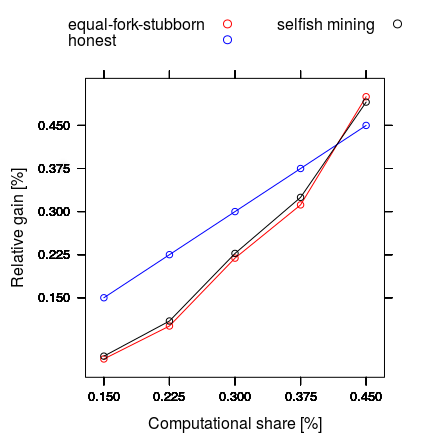
\includegraphics[width=12cm]{relative_block_share}
\centering
\caption{Relative revenue of the selfish miner}
\label{fig:relative_block_share}
\end{figure}

In figure \ref{fig:relative_block_share} the relative revenue, given a particular computation share and selfish mining strategy, is shown.
The graph shows that the two strategies selfish mining with \textit{lead stubborn, equal-fork stubborn} (\textit{L, F}) and selfish mining with all three modifications (\textit{L, F, T\textsubscript{1}}) are the worst performing strategies.
The relative share of accepted blocks of the two strategies stays clearly under the relative proportion which could be obtained by behaving honestly.
Also with an increase of the computational power the efficiency of the two selfish strategies is not amplified and the curve shows a linear progression.
The other six, better performing strategies are all exhibiting a similar behaviour.
The performance of these strategies is intensified with the augmentation of the computational share underlined by a concave curve.
Overall all selfish mining strategies are performing poorly and only with a computational share of about 40\% the six better performing strategies can retain a more significant share than the share obtained behaving honestly.
In table \ref{tab:relative_share_45} the relative  revenue share of the selfish miner with 45\% of computation power is shown.
The best performing strategies are equal-fork stubbornness (\textit{F}) and normal selfish mining (\textit{S}) followed by trail stubborn mining modified with equal-fork stubbornness \textit{F, T\textsubscript{1}} and the strategy trail stubborn (\textit{T\textsubscript{1}}).
These four strategies achieve almost similar results and are only 3\% apart.

\begin{table}
  \centering
  \begin{tabular}{cccc}
    \toprule
    strategy & share selfish & rank & difference to best\\
    \midrule
    F & 50\% & 1 & - \\
    S & 49.1\% & 2 & 0.9\% \\
    F, T\textsubscript{1} & 48.7\% & 3 & 1.3\% \\
    T\textsubscript{1} & 47\% & 4 & 3\% \\
    L & 45.4\% & 5 & 4.6\% \\
    L, T\textsubscript{1} & 45.3\% & 6 & 4.7\% \\
    H & 45\% & 7 & 5\% \\
    L, F, T\textsubscript{1} & 35.1\% & 8 & 14.9\% \\
    L, F & 33.8\% & 9 & 16.2\% \\
    \bottomrule
  \end{tabular}
  \caption{Relative share of selfish miner with 45\% of computational share}
  \label{tab:relative_share_45}
\end{table}

\begin{figure}[t]
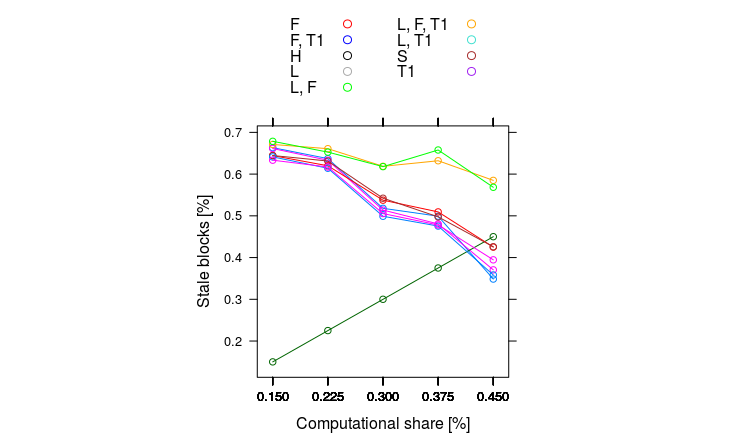
\includegraphics[width=12cm]{stale_blocks}
\centering
\caption{Share of stale blocks created by the selfish miner}
\label{fig:stale_blocks}
\end{figure}

Figure \ref{fig:stale_blocks} shows the share of stale blocks found by the selfish miner.
In the honest case, the share of created stale blocks increases linearly with the computational share.
Contrary to the line showing the honest behaviour proceed the lines depicting the different selfish mining strategies.
Especially if the computational share is low, over 60\% of the stale blocks of the network are created by the selfish miner.
With an increasing share of computational power, the share of stale blocks declines significantly, except the two strategies lead stubborn combined with equal-fork stubborn (\textit{L, F}) and selfish mining modified with all stubborn variations (\textit{L, F, T\textsubscript{1}}) which remain on the same level.
Additionally, the figure shows that only with a very high amount of computational share the selfish strategies are achieving better results than the normal, honest behaviour.

\begin{figure}[t]
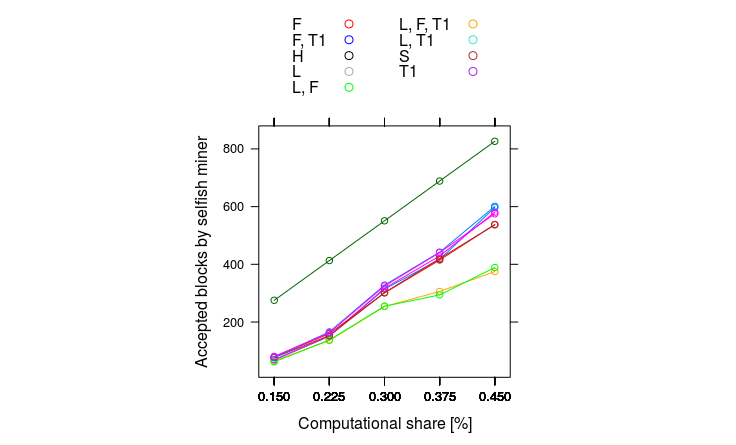
\includegraphics[width=12cm]{accepted_blocks_selfish}
\centering
\caption{Blocks created by the selfish miner and accepted in the longest chain}
\label{fig:accepted_blocks_selfish}
\end{figure}

The total amount of accepted blocks by the selfish miner, given a particular strategy and computational share, is shown in figure \ref{fig:accepted_blocks_selfish}.
The graph shows again the gap between the two bad performing strategies and the six other strategies which work slightly better.
Additionally, it can be seen that the absolute amount of accepted blocks during the execution of selfish mining is significantly lower than the number of blocks accepted when the nodes behave honestly.
Hence, in the short-run, all selfish mining strategies are yielding less mining rewards for the selfish miner than the normal, honest behaviour.

\begin{figure}[t]
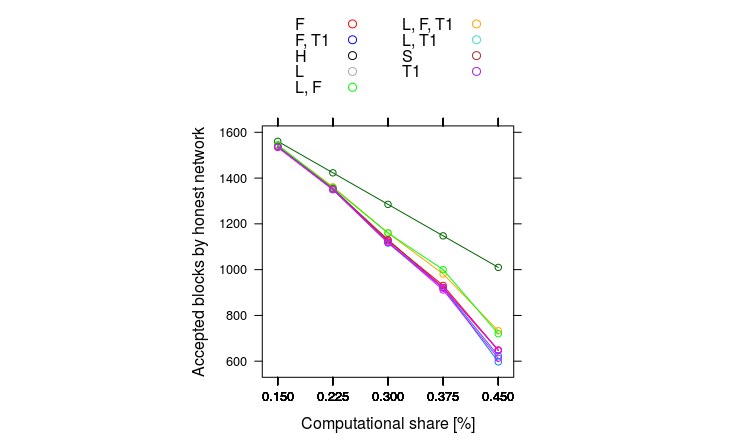
\includegraphics[width=12cm]{accepted_blocks_honest}
\centering
\caption{Blocks created by the honest network and accepted in the longest chain}
\label{fig:accepted_blocks_honest}
\end{figure}

The honest network also creates less accepted blocks during a selfish mining attack as shown in figure \ref{fig:accepted_blocks_honest}.
Since the selfish mining strategies are functioning better with an increasing computational share of the selfish miner, the gap between the case where all nodes behave honestly and the case where one node conducts selfish mining even increases.
The performance differences between the selfish mining strategies can also be seen in this figure.

\begin{figure}[t]
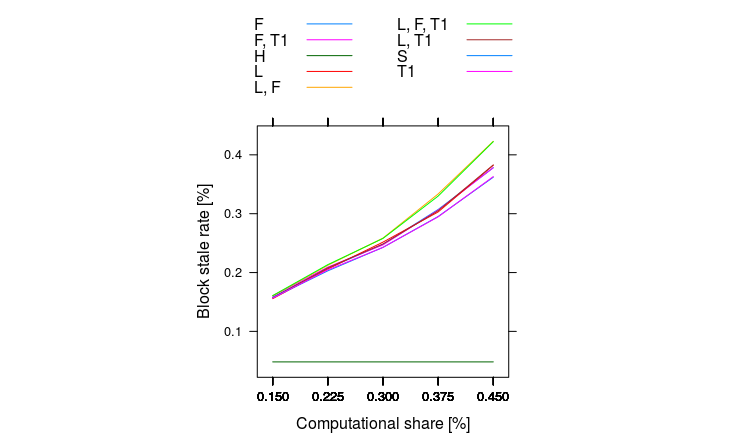
\includegraphics[width=12cm]{stale_rate}
\centering
\caption{Stale block rate}
\label{fig:stale_rate}
\end{figure}

Lastly, in figure \ref{fig:stale_rate} the relative amount of stale blocks in the network during the simulations is shown.
If all nodes behave honestly, the stale block rate is 4.821\% as measured during the evaluation of the simulation software.
In the case that a node conducts a selfish mining strategy the stale block rate is significantly higher and increases further if the computational power of the selfish miner is augmented.
Furthermore, the gap between the two worst performing selfish strategies and the other strategies can be observed.
If a node conducts lead stubbornness combined with equal-fork stubbornness (\textit{L, F}) or selfish mining with all three modifications (\textit{L, F, T\textsubscript{1}}), there are even more stale blocks in the network.

Similar as during the evaluation of the deterministic behaviour of the simulation software in chapter 45, also during the execution of the selfish mining scenarios the utilisation of the CPU and the memory of the host machine stayed under 10\% as shown in figure \ref{fig:selfish_simulations_cpu} and figure \ref{fig:selfish_simulations_memory}.
Thus, the specifications of the host machine did not restrict the simulations in any way.

\begin{figure}[t]
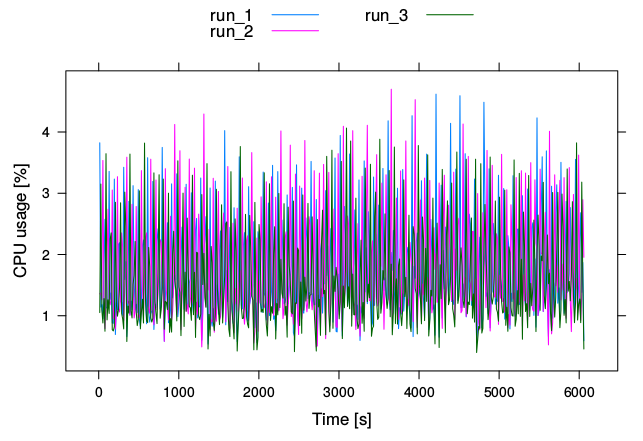
\includegraphics[width=8cm]{selfish_simulations_cpu}
\centering
\caption{CPU usage during the triple execution of a simulation scenario}
\label{fig:selfish_simulations_cpu}
\end{figure}

\begin{figure}[t]
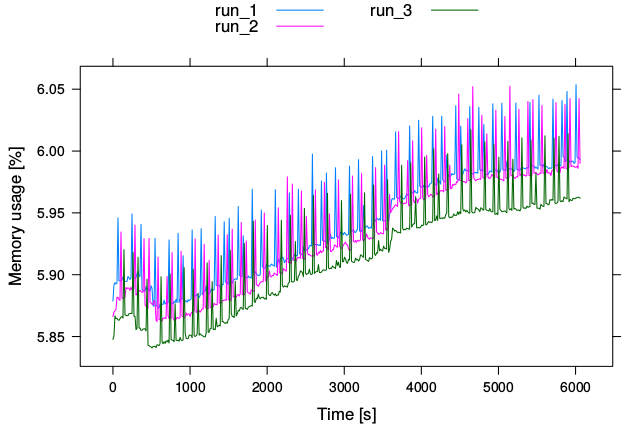
\includegraphics[width=8cm]{selfish_simulations_memory}
\centering
\caption{Memory usage during the triple execution of a simulation scenario}
\label{fig:selfish_simulations_memory}
\end{figure}


\chapter{Results}
\section{Installation}



\chapter{Discussion}
\section{Installation}



\chapter{Further research}
\section{Installation}



% Remove following line for the final thesis.
%% intro.tex
%% Copyright (C) 2014-2016 by Thomas Auzinger <thomas@auzinger.name>
%
% This work may be distributed and/or modified under the
% conditions of the LaTeX Project Public License, either version 1.3
% of this license or (at your option) any later version.
% The latest version of this license is in
%   http://www.latex-project.org/lppl.txt
% and version 1.3 or later is part of all distributions of LaTeX
% version 2005/12/01 or later.
%
% This work has the LPPL maintenance status `maintained'.
%
% The Current Maintainer of this work is Thomas Auzinger.
%
% This work consists of the files vutinfth.dtx and vutinfth.ins
% and the derived file vutinfth.cls.
% This work also consists of the file intro.tex.


\newacronym{ctan}{CTAN}{Comprehensive TeX Archive Network}
\newacronym{faq}{FAQ}{Frequently Asked Questions}
\newacronym{pdf}{PDF}{Portable Document Format}
\newacronym{svn}{SVN}{Subversion}
\newacronym{wysiwyg}{WYSIWYG}{What You See Is What You Get}

\newglossaryentry{texteditor}
{
  name={editor},
  description={A text editor is a type of program used for editing plain text files.}
}

\chapter{Introduction to \LaTeX}

Since \LaTeX\ is widely used in academia and industry, there exists a plethora of freely accessible introductions to the language.
Reading through the guide at \url{https://en.wikibooks.org/wiki/LaTeX} serves as a comprehensive overview for most of the functionality and is highly recommended before starting with a thesis in \LaTeX.

\section{Installation}

A full \LaTeX\ distribution\index{distribution} consists of not only of the binaries that convert the source files to the typeset documents, but also of a wide range of packages and their documentation.
Depending on the operating system, different implementations are available as shown in Table~\ref{tab:distrib}.
\textbf{Due to the large amount of packages that are in everyday use and due to their high interdependence, it is paramount to keep the installed distribution\index{distribution} up to date.}
Otherwise, obscure errors and tedious debugging ensue.

\begin{table}
  \centering
  \begin{tabular}{cccc}
    \toprule
    Distribution & Unix         & Windows      & MacOS        \\
    \midrule
    TeX Live     & \textbf{yes} & yes          & (yes)        \\
    MacTeX       & no           & no           & \textbf{yes} \\
    MikTeX       & no           & \textbf{yes} & no           \\
    \bottomrule
  \end{tabular}
  \caption{\TeX/\LaTeX\ distributions for different operating systems. Recomended choice in \textbf{bold}.}
  \label{tab:distrib} % \label has to be placed AFTER \caption to produce correct cross-references.
\end{table}

\section{Editors}

A multitude of \TeX\ \glspl{texteditor} are available differing in their editing models, their supported operating systems and their feature sets.
A comprehensive overview of \glspl{texteditor} can be found at the Wikipedia page  \url{https://en.wikipedia.org/wiki/Comparison_of_TeX_editors}.
TeXstudio (\url{http://texstudio.sourceforge.net/}) is recommended.
Most editors support the scrolling the typeset preview document to a location in the source document by \verb|Ctrl| clicking the location in the source document.

\section{Compilation}

Modern editors usually provide the compilation programs to generate \gls{pdf} documents and for most \LaTeX\ source files, this is sufficient.
More advanced \LaTeX\ functionality, such as glossaries and bibliographies, needs additional compilation steps, however.
It is also possible that errors in the compilation process invalidate intermediate files and force subsequent compilation runs to fail.
It is advisable to delete intermediate files (\verb|.aux|, \verb|.bbl|, etc.), if errors occur and persist.
All files that are not generated by the user are automatically regenerated.
To compile the current document, the steps as shown in Table~\ref{tab:compile} have to be taken.


\begin{table}
  \centering
  \begin{tabular}{rl}
    \toprule
    & Description \\
    \midrule
    1 & Scan for refs, toc/lof/lot/loa items and cites \\
    2 & Build the bibliography     \\
    3 & Link refs and build the toc/lof/lot/loa \\
    4 & Link the bibliography \\
    5 & Build the glossary \\
    6 & Build the acronyms \\
    7 & Build the index \\
    8 & Link the glossary, acronyms, and the index \\
    9 & Link the bookmarks \\
    \midrule
    & Command \\
    \midrule
    1 & \verb|pdflatex.exe  example| \\
    2 & \verb|bibtex.exe    example| \\
    3 & \verb|pdflatex.exe  example| \\
    4 & \verb|pdflatex.exe  example| \\
    5 & \verb|makeindex.exe -t example.glg -s example.ist| \\
      & \verb|              -o example.gls example.glo| \\
    6 & \verb|makeindex.exe -t example.alg -s example.ist| \\
      & \verb|              -o example.acr example.acn| \\
    7 & \verb|makeindex.exe -t example.ilg -o example.ind example.idx| \\
    8 & \verb|pdflatex.exe  example| \\
    9 & \verb|pdflatex.exe  example| \\
    \bottomrule
  \end{tabular}
  \caption{Compilation steps for this document. The following abbreviations were used: table of contents (toc), list of figures (lof), list of tables (lot), list of algorithms (loa).}
  \label{tab:compile} % \label has to be placed AFTER \caption to produce correct cross-references.
\end{table}


\section{Basic Functionality}

In this section, various examples are given of the fundamental building blocks used in a thesis.
Many \LaTeX\ commands have a rich set of options that can be supplied as optional arguments.
The documentation of each command should be consulted to get an impression of the full spectrum of its functionality.

\subsection{Floats}

Two main categories of page elements can be differentiated in the usual \LaTeX\ workflow: \textit{(i)} the main stream of text and \textit{(ii)} floating containers that are positioned at convenient positions throughout the document.
In most cases, tables, plots, and images are put into such containers since they are usually positioned at the top or bottom of pages.
These are realized by the two environments \verb|figure| and \verb|table|, which also provide functionality for cross-referencing (see Table~\ref{tab:intro} and Figure~\ref{fig:intro}) and the generation of corresponding entries in the list of figures and the list of tables.
Note that these environments solely act as containers and can be assigned arbitrary content.

\subsection{Tables}

A table in \LaTeX\ is created by using a \verb|tabular| environment or any of its extensions, e.g., \verb|tabularx|.
The commands \verb|\multirow| and \verb|\multicolumn| allow table elements to span multiple rows and columns.

\begin{table}[h] % placement specifier
  \centering
  \begin{tabular}{lll}
    \toprule
    \multicolumn{2}{c}{Position} \\
    \cmidrule{1-2} % partial horizontal rule
    Group & Abbrev & Name \\
    \midrule
    Goalkeeper & GK & Paul Robinson \\
    \midrule
    \multirow{4}{*}{Defenders} & LB & Lucus Radebe \\
                               & DC & Michael Duburry \\
                               & DC & Dominic Matteo \\
                               & RB & Didier Domi \\
    \midrule
    \multirow{3}{*}{Midfielders} & MC & David Batty \\
                                 & MC & Eirik Bakke \\
                                 & MC & Jody Morris \\
    \midrule
    Forward & FW & Jamie McMaster \\
    \midrule
    \multirow{2}{*}{Strikers} & ST & Alan Smith \\
                              & ST & Mark Viduka \\
    \bottomrule
  \end{tabular}
  \caption{Adapted example from the \LaTeX guide at \url{https://en.wikibooks.org/wiki/LaTeX/Tables}. This example uses rules specific to the \texttt{booktabs} package and employs the multi-row functionality of the \texttt{multirow} package.}
  \label{tab:intro} % \label has to be placed AFTER \caption to produce correct cross-references.
\end{table}

\subsection{Images}

An image is added to a document via the \verb|\includegraphics| command as shown in Figure~\ref{fig:intro}.
The \verb|\subcaption| command can be used to reference subfigures, such as Figure~\ref{fig:intro:full width} and~\ref{fig:intro:half width}.

\begin{figure}[h]
  \centering
  \begin{subfigure}[b]{0.45\columnwidth}
    \centering
    
\includegraphics[width=\textwidth]{TU_INF_Logo_gray}
    \subcaption{The header logo at text width.}
    \label{fig:intro:full width}
  \end{subfigure}
  \begin{subfigure}[b]{0.45\columnwidth}
    \centering
    
\includegraphics[width=0.5\textwidth]{TU_INF_Logo_gray}
    \subcaption{The header logo at half the text width.}
    \label{fig:intro:half width}
  \end{subfigure}
  \caption{The header logo at different sizes.}
  \label{fig:intro} % \label has to be placed AFTER \caption (or \subcaption) to produce correct cross-references.
\end{figure}

\subsection{Mathematical Expressions}

One of the original motivation to create the \TeX\ system was the need for mathematical typesetting.
To this day, \LaTeX\ is the preferred system to write math-heavy documents and a wide variety of functions aids the author in this task.
A mathematical expression can be inserted inline as $\sum_{n=1}^{\infty} \frac{1}{n^2} = \frac{\pi^2}{6}$ outside of the text stream as \[ \sum_{n=1}^{\infty} \frac{1}{n^2} = \frac{\pi^2}{6} \] or as numbered equation with
\begin{equation}
\sum_{n=1}^{\infty} \frac{1}{n^2} = \frac{\pi^2}{6}.
\end{equation}

\subsection{Pseudo Code}

The presentation of algorithms can be achieved with various packages; the most popular are \verb|algorithmic|, \verb|algorithm2e|, \verb|algorithmicx|, or \verb|algpseudocode|.
An overview is given at \url{https://tex.stackexchange.com/questions/229355}.
An example of the use of the \verb|alogrithm2e| package is given with Algorithm~\ref{alg:gauss-seidel}.

\begin{algorithm}
  \SetKw{BreakFor}{break for}
  \KwIn{A scalar~$\epsilon$, a matrix $\mathbf{A} = (a_{ij})$, a vector $\vec{b}$, and an initial vector $\vec{x}^{(0)}$}
  \KwOut{$\vec{x}^{(n)}$ with $\mathbf{A} \vec{x}^{(n)} \approx \vec{b}$}
  \For{$k\leftarrow 1$ \KwTo maximum iterations}
  {
     \For{$i\leftarrow 1$ \KwTo $n$}
     {
        $x_i^{(k)} = \frac{1}{a_{ii}} \left(b_i-\sum_{j<i} a_{ij} x_j^{(k)} - \sum_{j>i} a_{ij} x_j^{(k-1)} \right)$\;
     }
     \If{$\lvert\vec{x}^{(k)}-\vec{x}^{(k-1)}\rvert < \epsilon$}
     {\BreakFor\;}
  }
  \Return{$\vec{x}^{(k)}$\;}
  \caption{Gauss-Seidel}
  \label{alg:gauss-seidel} % \label has to be placed AFTER \caption to produce correct cross-references.
\end{algorithm}

\section{Bibliography}

The referencing of prior work is a fundamental requirement of academic writing and well supported by \LaTeX.
The \textsc{Bib}\TeX\ reference management software is the most commonly used system for this purpose.
Using the \verb|\cite| command, it is possible to reference entries in a \verb|.bib| file out of the text stream, e.g., as~\cite{Turing1936}.
The generation of the formatted bibliography needs a separate execution of \verb|bibtex.exe| (see Table~\ref{tab:compile}).

\section{Table of Contents}

The table of contents is automatically built by successive runs of the compilation, e.g., of \verb|pdflatex.exe|.
The command \verb|\setsecnumdepth| allows the specification of the depth of the table of contents and additional entries can be added to the table of contents using \verb|\addcontentsline|.
The starred versions of the sectioning commands, i.e., \verb|\chapter*|, \verb|\section*|, etc., remove the corresponding entry from the table of contents.

\section{Acronyms / Glossary / Index}

The list of acronyms, the glossary, and the index need to be built with a separate execution of \verb|makeindex| (see Table~\ref{tab:compile}).
Acronyms have to be specified with \verb|\newacronym| while glossary entries use \verb|\newglossaryentry|.
Both are then used in the document content with one of the variants of \verb|\gls|, such as \verb|\Gls|, \verb|\glspl|, or \verb|\Glspl|.
Index items are simply generated by placing \verb|\index|\marg{entry} next to all the words that correspond to the index entry \meta{entry}.
Note that many enhancements exist for these functionalities and the documentation of the \verb|makeindex| and the \verb|glossaries| packages should be consulted.

\section{Tips}

Since \TeX\ and its successors do not employ a \gls{wysiwyg} editing scheme, several guidelines improve the readability of the source content:
\begin{itemize}
\item Each sentence in the source text should start with a new line.
      This helps not only the user navigation through the text, but also enables revision control systems (e.g. \gls{svn}, Git) to show the exact changes authored by different users.
      Paragraphs are separated by one (or more) empty lines.
\item Environments, which are defined by a matching pair of \verb|\begin{name}| and \verb|\end{name}|, can be indented by whitespace to show their hierarchical structure.
\item In most cases, the explicit use of whitespace (e.g. by adding \verb|\hspace{4em}| or \verb|\vspace{1.5cm}|) violates typographic guidelines and rules.
      Explicit formatting should only be employed as a last resort and, most likely, better ways to achieve the desired layout can be found by a quick web search.
\item The use of bold or italic text is generally not supported by typographic considerations and the semantically meaningful \verb|\emph{|\texttt{$\dots$}\verb|}| should be used.
\end{itemize}

The predominant application of the \LaTeX\ system is the generation of \gls{pdf} files via the \textsc{Pdf}\LaTeX\ binaries.
In the current version of \textsc{Pdf}\LaTeX, it is possible that absolute file paths and user account names are embedded in the final \gls{pdf} document.
While this poses only a minor security issue for all documents, it is highly problematic for double blind reviews.
The process shown in Table~\ref{tab:ps2pdf} can be employed to strip all private information from the final \gls{pdf} document.

\begin{table}[h]
  \centering
  \begin{tabular}{rl}
  \toprule
  & Command \\
  \midrule
  1 & Rename the \gls{pdf} document \verb|final.pdf| to \verb|final.ps|. \\
  2 & Execute the following command: \\
    & \verb|ps2pdf -dPDFSETTINGS#/prepress ^| \\
    & \verb| -dCompatibilityLevel#1.4 ^| \\
    & \verb| -dAutoFilterColorImages#false ^| \\
    & \verb| -dAutoFilterGrayImages#false ^| \\
    & \verb| -dColorImageFilter#/FlateEncode ^| \\
    & \verb| -dGrayImageFilter#/FlateEncode ^| \\
    & \verb| -dMonoImageFilter#/FlateEncode ^| \\
    & \verb| -dDownsampleColorImages#false ^| \\
    & \verb| -dDownsampleGrayImages#false ^| \\
    & \verb| final.ps final.pdf| \\
  \bottomrule
  \end{tabular}

  On Unix-based systems, replace \verb|#| with \verb|=| and \verb|^| with \verb|\|.
  \caption{Anonymization of \gls{pdf} documents.}
  \label{tab:ps2pdf}
\end{table}

\section{Resources}

\subsection{Useful Links}

In the following, a listing of useful web resources is given.
\begin{description}
\item[\url{https://en.wikibooks.org/wiki/LaTeX}] An extensive wiki-based guide to \LaTeX.
\item[\url{http://www.tex.ac.uk/faq}] A (huge) set of \gls{faq} about \TeX\ and \LaTeX.
\item[\url{https://tex.stackexchange.com/}] The definitive user forum for non-trivial \LaTeX-related questions and answers.
\end{description}

\subsection[Comprehensive TeX Archive Network]{\gls{ctan}}

The \gls{ctan} is the official repository for all \TeX\ related material.
It can be accessed via \url{https://www.ctan.org/} and hosts (among other things) a huge variety of packages that provide extended functionality for \TeX\ and its successors.
Note that most packages contain \gls{pdf} documentation that can be directly accessed via \gls{ctan}.

In the following, a short, non-exhaustive list of relevant \gls{ctan}-hosted packages is given together with their relative path.
\begin{description}[itemsep=0ex]
\item[\href{https://www.ctan.org/pkg/algorithm2e}{algorithm2e}] Functionality for writing pseudo code.
\item[\href{https://www.ctan.org/pkg/amsmath}{amsmath}] Enhanced functionality for typesetting mathematical expressions.
\item[\href{https://www.ctan.org/pkg/amsfonts}{amssymb}] Provides a multitude of mathematical symbols.
\item[\href{https://www.ctan.org/pkg/booktabs}{booktabs}] Improved typesetting of tables.
\item[\href{https://www.ctan.org/pkg/enumitem}{enumitem}] Control over the layout of lists (\verb|itemize|, \verb|enumerate|, \verb|description|).
\item[\href{https://www.ctan.org/pkg/fontenc}{fontenc}] Determines font encoding of the output.
\item[\href{https://www.ctan.org/pkg/glossaries}{glossaries}] Create glossaries and list of acronyms.
\item[\href{https://www.ctan.org/pkg/graphicx}{graphicx}] Insert images into the document.
\item[\href{https://www.ctan.org/pkg/inputenc}{inputenc}] Determines encoding of the input.
\item[\href{https://www.ctan.org/pkg/l2tabu}{l2tabu}] A description of bad practices when using \LaTeX.
\item[\href{https://www.ctan.org/pkg/mathtools}{mathtools}] Further extension of mathematical typesetting.
\item[\href{https://www.ctan.org/pkg/memoir}{memoir}] The document class on upon which the \verb|vutinfth| document class is based.
\item[\href{https://www.ctan.org/pkg/multirow}{multirow}] Allows table elements to span several rows.
\item[\href{https://www.ctan.org/pkg/pgfplots}{pgfplots}] Function plot drawings.
\item[\href{https://www.ctan.org/pkg/pgf}{pgf/TikZ}] Creating graphics inside \LaTeX\ documents.
\item[\href{https://www.ctan.org/pkg/subcaption}{subcaption}] Allows the use of subfigures and enables their referencing.
\item[\href{https://www.ctan.org/tex-archive/info/symbols/comprehensive/}{symbols/comprehensive}] A listing of around 5000 symbols that can be used with \LaTeX.
\item[\href{https://www.ctan.org/pkg/voss-mathmode}{voss-mathmode}] A comprehensive overview of typesetting mathematics in \LaTeX.
\item[\href{https://www.ctan.org/pkg/xcolor}{xcolor}] Allows the definition and use of colors.
\end{description} % A short introduction to LaTeX.

\backmatter

% Use an optional list of figures.
\listoffigures % Starred version, i.e., \listoffigures*, removes the toc entry.

% Use an optional list of tables.
\cleardoublepage % Start list of tables on the next empty right hand page.
\listoftables % Starred version, i.e., \listoftables*, removes the toc entry.

% Use an optional list of alogrithms.
\listofalgorithms
\addcontentsline{toc}{chapter}{List of Algorithms}

% Add an index.
\printindex

% Add a glossary.
\printglossaries

% Add a bibliography.
\bibliographystyle{alpha}
\bibliography{intro}

\end{document}